%%%%%%%%%%%%%%%%%%%%%%%%%%%%%%%%%%%%%%%%%%%%%%%%%%%%%%%%%%%%%%%
%
% Welcome to writeLaTeX --- just edit your LaTeX on the left,
% and we'll compile it for you on the right. If you give
% someone the link to this page, they can edit at the same
% time. See the help menu above for more info. Enjoy!
%
%%%%%%%%%%%%%%%%%%%%%%%%%%%%%%%%%%%%%%%%%%%%%%%%%%%%%%%%%%%%%%%

% --------------------------------------------------------------
% This is all preamble stuff that you don't have to worry about.
% Head down to where it says "Start here"
% --------------------------------------------------------------
 
\documentclass[12pt]{article}
 
\usepackage[margin=1in]{geometry}
\usepackage{amsmath,amsthm,amssymb}

\usepackage{listings}
\usepackage{xcolor}
\usepackage{circuitikz}
\usetikzlibrary{bending}
\usetikzlibrary{patterns,decorations.pathmorphing,positioning}
\usepackage{enumitem}

%New colors defined below
\definecolor{codegreen}{rgb}{0,0.6,0}
\definecolor{codegray}{rgb}{0.5,0.5,0.5}
\definecolor{codepurple}{rgb}{0.58,0,0.82}
\definecolor{backcolour}{rgb}{0.95,0.95,0.92}

%Code listing style named "mystyle"
\lstdefinestyle{mystyle}{
  backgroundcolor=\color{backcolour}, commentstyle=\color{codegreen},
  keywordstyle=\color{magenta},
  numberstyle=\tiny\color{codegray},
  stringstyle=\color{codepurple},
  basicstyle=\ttfamily\footnotesize,
  breakatwhitespace=false,         
  breaklines=true,                 
  captionpos=b,                    
  keepspaces=true,                 
  numbers=left,                    
  numbersep=5pt,                  
  showspaces=false,                
  showstringspaces=false,
  showtabs=false,                  
  tabsize=2
}

%"mystyle" code listing set
\lstset{style=mystyle}

 
\newcommand{\N}{\mathbb{N}}
\newcommand{\Z}{\mathbb{Z}}
 
\newenvironment{theorem}[2][Theorem]{\begin{trivlist}
\item[\hskip \labelsep {\bfseries #1}\hskip \labelsep {\bfseries #2.}]}{\end{trivlist}}
\newenvironment{lemma}[2][Lemma]{\begin{trivlist}
\item[\hskip \labelsep {\bfseries #1}\hskip \labelsep {\bfseries #2.}]}{\end{trivlist}}
\newenvironment{exercise}[2][Exercise]{\begin{trivlist}
\item[\hskip \labelsep {\bfseries #1}\hskip \labelsep {\bfseries #2.}]}{\end{trivlist}}
\newenvironment{problem}[2][Problem]{\begin{trivlist}
\item[\hskip \labelsep {\bfseries #1}\hskip \labelsep {\bfseries #2.}]}{\end{trivlist}}
\newenvironment{question}[2][Question]{\begin{trivlist}
\item[\hskip \labelsep {\bfseries #1}\hskip \labelsep {\bfseries #2.}]}{\end{trivlist}}
\newenvironment{corollary}[2][Corollary]{\begin{trivlist}
\item[\hskip \labelsep {\bfseries #1}\hskip \labelsep {\bfseries #2.}]}{\end{trivlist}}

\newenvironment{solution}{\begin{proof}[Solution]}{\end{proof}}
 
\begin{document}
 
% --------------------------------------------------------------
%                         Start here
% --------------------------------------------------------------
 
\title{Test 1}%replace X with the appropriate number
\author{Mengxiang Jiang\\ %replace with your name
EEEN 5338 Digital and DSP Based Control} %if necessary, replace with your course title
 
\maketitle
 
\begin{problem}{1} %You can use theorem, exercise, problem, or question here.  Modify x.yz to be whatever number you are proving
As per our review of pre-requisite materials in class and our brief discussions related to the following, find the mathematical models (differential equations) for the following systems:\\
\begin{circuitikz} \draw
    (0,4) to[battery, l=$e_i(t)$] (0,0) -- (4,0)
    to [resistor, l=$4\Omega$] (4,4)
    to [capacitor, l=$\frac{1}{8}F$] (0,4)
    (8,4) to [inductor, l=$2H$] (4,4)
    (8,4) to [resistor, l=$4\Omega$] (8,0)
    (8,0) -- (4,0);
    \draw[thin, <-] (2,2)node{$i_1$}  ++(-45:1) arc (-45:135:1);
    \draw[thin, <-] (6,2)node{$i_2$}  ++(-45:1) arc (-45:135:1);
  \end{circuitikz}
  \begin{align*}
    e_i = \frac{1}{C}\int{i_1dt}+R_1(i_1-i_2) = 8\int{i_1dt} + 4(i_1-i_2)\\
    \implies \dot{e_i} = 8i_1+4\frac{di_1}{dt}-4\frac{di_2}{dt}\\
    R_1(i_2-i_1)+L\frac{di_2}{dt}+R_2(i_2)=4(i_2-i_1) + 2\frac{di_2}{dt}+4i_2=0\\
    \implies 8i_2+2\frac{di_2}{dt} = 4i_1 \implies 4i_2 + \frac{di_2}{dt} = 2i_1\\
    e_A = R_1(i_2-i_1) = 4i_2-4i_1\\
    \implies \dot{e_A} = 4\frac{di_2}{dt} - 4\frac{di_1}{dt}\\
    \implies \dot{e_i} = 8i_1-\dot{e_A}\\
    e_o = R_2(-i_2) = -4i_2\\
    \implies 2i_1=-e_o-\frac{1}{4}\dot{e_o}\\
    \implies \dot{e_i} = -4e_o-\dot{e_o} - \dot{e_A}\\
  \end{align*}
  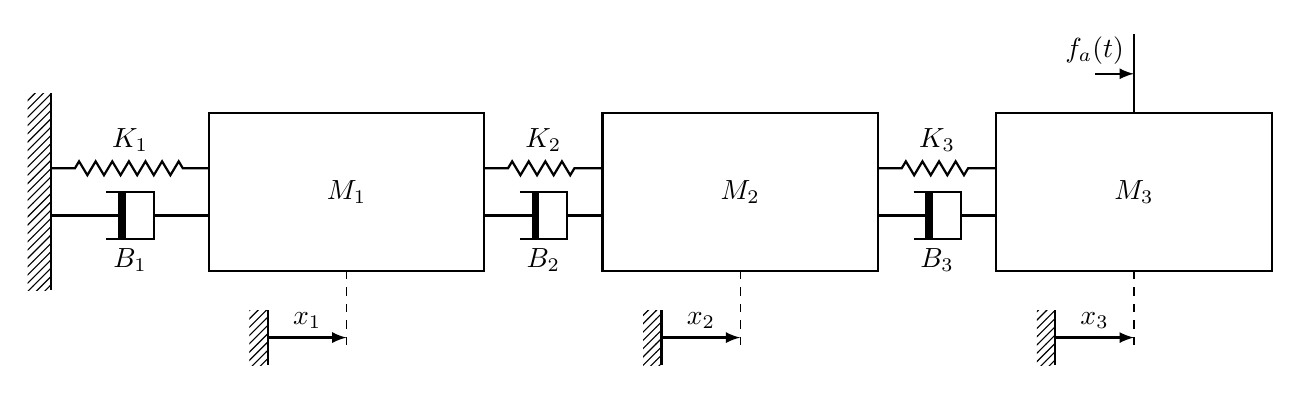
\begin{tikzpicture}[every node/.style={outer sep=0pt},thick,
    mass/.style={draw,thick},
    spring/.style={thick,decorate,decoration={zigzag,pre length=0.3cm,post
    length=0.3cm,segment length=6}},
    ground/.style={fill,pattern=north east lines,draw=none,minimum
    width=0.75cm,minimum height=0.3cm},
    dampic/.pic={\fill[white] (-0.1,-0.3) rectangle (0.3,0.3);
    \draw (-0.3,0.3) -| (0.3,-0.3) -- (-0.3,-0.3);
    \draw[line width=1mm] (-0.1,-0.3) -- (-0.1,0.3);}]
   
     \node[mass,minimum width=3.5cm,minimum height=2cm] (m1) {$M_1$};
     \node[mass,minimum width=3.5cm,minimum height=2cm,right=1.5cm of
     m1] (m2) {$M_2$};
     \node[mass,minimum width=3.5cm,minimum height=2cm,right=1.5cm of
     m2] (m3) {$M_3$};
     \node[left=2cm of m1,ground,minimum width=3mm,minimum height=2.5cm] (g1){};
     \draw (g1.north east) -- (g1.south east);
   
     \draw[spring] ([yshift=3mm]g1.east) coordinate(aux)
      -- (m1.west|-aux) node[midway,above=1mm]{$K_1$};
     \draw[spring]  (m1.east|-aux) -- (m2.west|-aux) node[midway,above=1mm]{$K_2$};
     \draw[spring]  (m2.east|-aux) -- (m3.west|-aux) node[midway,above=1mm]{$K_3$};
   
     \draw ([yshift=-3mm]g1.east) coordinate(aux')
      -- (m1.west|-aux') pic[midway]{dampic} node[midway,below=3mm]{$B_1$}
        (m1.east|-aux') -- (m2.west|-aux') pic[midway]{dampic} node[midway,below=3mm]{$B_2$}
        (m2.east|-aux') -- (m3.west|-aux') pic[midway]{dampic} node[midway,below=3mm]{$B_3$};
   
    \foreach \X in {1,2,3}  
    {
        \draw[thin,dashed] (m\X.south) -- ++ (0,-1) coordinate[pos=0.85](aux'\X);
        \draw[latex-] (aux'\X) -- ++ (-1,0) node[midway,above]{$x_\X$}
        node[left,ground,minimum height=7mm,minimum width=1mm] (g'\X){};
        \draw[thick] (g'\X.north east) -- (g'\X.south east);
    }
    \draw[thin] (m3.north) -- ++ (0,1) coordinate[midway](aux2);
    \draw[latex-] (aux2) -- ++ (-0.5,0) node[above]{$f_a(t)$}; 
   \end{tikzpicture}
   \begin{align*}
    -B_1\dot{x_1}-K_1x_1+K_2(x_2-x_1)+B_2(\dot{x_2}-\dot{x_1})=M_1\ddot{x_1}\\
    -B_2(\dot{x_2}-\dot{x_1})-K_2(x_2-x_1)+B_3(\dot{x_3}-\dot{x_2}) = M_2\ddot{x_2}\\
    -B_3(\dot{x_3}-\dot{x_2})-K_3(x_3-x_2)+f_a = M_3\ddot{x_3}
   \end{align*}
\end{problem}
\pagebreak
\begin{problem}{2}
    For the following equations, determine:\\
    a) order?, b) linear?, c) time-invariant?, d) homogeneous?
    \begin{enumerate}[label=\roman*]
        \item $y(k+3) + 0.2y(k+1) + 0.01y(k)=0$\\
        The equation is 3rd order from the difference of $k+3$ and $k$.\\
        It is linear, since all the functions are linear.\\
        It is time-invariant because all the coefficients are constant.\\
        It is homogeneous since $u(k)$ is 0.
        \item $y(k+2) + e^{-0.2k}y(k+1) + 0.1y(k) = u(k)$\\
        The equation is 2nd order from the difference of $k+2$ and $k$.\\
        It is linear, since all the functions are linear.\\
        It is not time-invariant, since $e^{-0.2k}$ is not a constant coefficient.\\
        It is not homogeneous, since $u(k)$ is not 0.
        \item $y(k+5) + y(k+1) + 0.1y^3(k)=0.1u(k)$\\
        The equation is 5th order from the difference between $k+5$ and $k$.\\
        It is not linear, since $y^3$ is not a linear function.\\
        It is time-invariant because all the coefficients are constant.\\
        It is not homogeneous, since $u(k)$ is not 0.
    \end{enumerate}
\end{problem}
\pagebreak
\begin{problem}{3}
    Solve the following difference equations.
    \begin{enumerate}[label=\roman*]
        \item $y(k+1)-0.8y(k) = 1(k),\;y(0)=0$\\
        \begin{align*}
            zY(z)-0.8Y(z)=\frac{z}{z-1}\\
            Y(z)=\frac{z}{(z-0.8)(z-1)}\\
            z\left(\frac{1}{(z-0.8)(z-1)}\right)=z\left(\frac{A}{z-0.8}+\frac{B}{z-1}\right)\\
            1 = (z-1)A + (z-0.8)B\\
            z=1\implies 1=0.2B \implies B=5\\
            z=0.8\implies 1=-0.2A \implies A=-5\\
            Y(z)=\frac{-5z}{z-0.8} + \frac{5z}{z-1}\\
            f(k)=-5(0.8)^k + 5,\;k\in \N
        \end{align*}
        \item $y(k+1) - 0.8y(k)=1(k),\;y(0)=1$\\
        \begin{align*}
            zY(z)-z-0.8Y(z)=\frac{z}{z-1}\\
            Y(z)=\frac{z}{z-0.8}+\frac{z}{(z-0.8)(z-1)}\\
            \text{from partial fraction decomposition of part i we get:}\\
            Y(z)=\frac{z}{z-0.8}+\frac{-5z}{z-0.8} + \frac{5z}{z-1}=\frac{-4z}{z-0.8} + \frac{5z}{z-1}\\
            f(k)=-4(0.8)^k + 5,\;k\in \N
        \end{align*}
        \pagebreak
        \item $y(k+2)+0.7y(k+1)+0.06y(k)=\delta(k),\; y(0)=0,\;y(1)=2$\\
        \begin{align*}
            z^2Y(z)+0.7zY(z)+0.06Y(z)=1+2z\\
            \frac{Y(z)}{z}=\frac{2z+1}{z(z+0.1)(z+0.6)}\\
            \frac{2z+1}{z(z+0.1)(z+0.6)} = \frac{A}{z} + \frac{B}{z+0.1}+\frac{C}{z+0.6}\\
            2z+1=(z+0.1)(z+0.6)A+z(z+0.6)B+z(z+0.1)C\\
            z=0\implies 1 = 0.06A \implies A = \frac{100}{6}=\frac{50}{3}\\
            z=-0.1\implies 0.8 = -0.05B \implies B = -16\\
            z=-0.6\implies -0.2 = 0.3C\implies C = -\frac{2}{3}\\
            \frac{Y(z)}{z}=\frac{\frac{50}{3}}{z} + \frac{-16}{z+0.1} + \frac{-\frac{2}{3}}{z+0.6}\\
            Y(z)=\frac{50}{3} +\frac{-16z}{z+0.1}+\frac{-\frac{2}{3}z}{z+0.6}\\
            f(k)=\frac{50}{3}\delta(k) -16(-0.1)^k-\frac{2}{3}(-0.6)^k,\;k\in \N
        \end{align*}
    \end{enumerate}
\end{problem}
\pagebreak
\begin{problem}{4}
    Given:
    $$ y(k+1) -ay(k)=u(k),\;y(0)=0$$
    Find the impulse response h(k):
    \begin{enumerate}[label=\alph*)]
        \item From the difference equation
        \begin{align*}
            k = 0 \implies y(1) - ay(0) = 1 \implies y(1) = 1\\
            k = 1 \implies y(2) - ay(1) = 0 \implies y(2) = ay(1) = a\\
            k = 2 \implies y(3) - ay(2) = 0 \implies y(3) = ay(2) = a^2\\
            \implies y(k) = a^{k-1}\\
            g(k) = \begin{cases}
                a^{k-1} & k \geq 1\\
                0 & k < 1
            \end{cases}
        \end{align*}
        \item Using Z-transformation
        \begin{align*}
            zY(z) -aY(z) = U(z)\\
            G(z) = \frac{Y(z)}{U(z)} = \frac{1}{z-a} = z^{-1}\frac{z}{z-a}\\
            g(k) = \begin{cases}
                a^{k-1} & k \geq 1\\
                0 & k < 1
            \end{cases}
        \end{align*}
    \end{enumerate}
\end{problem}
\pagebreak
\begin{problem}{5}
    Given:
    $$y(k+1)-y(k)=u(k+1),\;y(0)=0$$
    Find the system transfer function and its response to a sampled unit step.
    \begin{align*}
        zY(z) - Y(z) = zU(z)\\
        \text{transfer function: }H(z) = \frac{Y(z)}{U(z)} = \frac{z}{z-1}\\
        \text{The $z$-transform of the sampled unit step $1(k)$ is also: } \frac{z}{z-1}\\
        \text{We multiply both to get: } \frac{z^2}{(z-1)^2} = z\frac{z}{(z-1)^2}\\
        \text{Applying the inverse $z$-transform:}\\
        y(i) = \begin{cases}
            i+1 & i \geq 0\\
            0 & i < 0
        \end{cases}
    \end{align*}
\end{problem}
% --------------------------------------------------------------
%     You don't have to mess with anything below this line.
% --------------------------------------------------------------
 
\end{document}